\section{Audio and Speech Coding}


\begin{questionbox}{Domanda 39}
Explain masking in the auditory system: define frequency masking and temporal masking (pre/post-masking) with their time-scale orders of magnitude.
\end{questionbox}


\begin{itemize}
  \item \textbf{Auditory masking} $\rightarrow$ strong sound makes weaker sound inaudible.
  \item \textbf{Codec use} $\rightarrow$ hide quantization noise below masking threshold.
  \item \textbf{Frequency masking} $\rightarrow$ simultaneous masking; strong component at $f_0$ raises threshold around nearby frequencies, mostly same critical band.
  \item \textbf{Temporal masking}:
  \begin{itemize}
    \item \textbf{pre-masking} $\rightarrow$ few ms before masker;
    \item \textbf{post-masking} $\rightarrow$ up to about $100$-$200$ ms after masker, depending on level/content.

  \end{itemize}
\end{itemize}
\begin{questionbox}{Domanda 40}
What is the critical band and how does it relate to the audibility condition of a set of sinusoids close in frequency?
\end{questionbox}


\begin{itemize}
  \item \textbf{Critical band} $\rightarrow$ frequency interval processed roughly by same cochlear auditory filter.
  \item Bandwidth increases with center frequency.
  \item Close sinusoids interact inside same band.
  \item \textbf{Audibility condition}:

\end{itemize}
$$
\sum_i g_i^2 > S_0(f_n)
$$

\begin{itemize}
  \item $g_i^2$ $\rightarrow$ sinusoid powers.
  \item $S_0(f_n)$ $\rightarrow$ absolute hearing threshold near frequency $f_n$.

\end{itemize}
\begin{questionbox}{Domanda 41}
(A\&S Comp.) Explain the dif and only iference between Source-Based (Parametric) coding and Sink-Based (Perceptual) coding.
\end{questionbox}


\begin{itemize}
  \item \textbf{Source-based / parametric coding} $\rightarrow$ models signal production.
  \begin{itemize}
    \item \textbf{Speech} $\rightarrow$ source-filter model of vocal folds + vocal tract.
    \item \textbf{Goal} $\rightarrow$ intelligibility and low latency at very low bitrate.
  \end{itemize}
  \item \textbf{Sink-based / perceptual coding} $\rightarrow$ models listener perception.
  \begin{itemize}
    \item \textbf{Audio codecs} $\rightarrow$ auditory masking + critical bands.
    \item \textbf{Goal} $\rightarrow$ transparent quality by removing inaudible information.

  \end{itemize}
\end{itemize}
\begin{questionbox}{Domanda 42}
(A\&S Comp.) Describe the “Analysis-by-Synthesis” (AbS) loop used in CELP (Code Excited Linear Prediction) codecs and why it represents an improvement over simple LPC-10.
\end{questionbox}


\begin{itemize}
  \item \textbf{LPC-10} $\rightarrow$ simplified excitation: impulse train for voiced, noise for unvoiced $\rightarrow$ synthetic sound.
  \item \textbf{CELP} $\rightarrow$ \textbf{Analysis-by-Synthesis} closed-loop search:

\end{itemize}
\begin{figure}[H]
\centering
\begin{tikzpicture}[
    block/.style={draw, rectangle, minimum width=2.4cm, minimum height=0.8cm, align=center, rounded corners=3pt, fill=purple!10, draw=purple!50!black, font=\small},
    arrow/.style={-latex, thick, draw=purple!50!black}
]
    \node [block] (exc) {Candidate codebook\\excitation};
    \node [block, right=0.8cm of exc] (gain) {Gain};
    \node [block, right=0.8cm of gain] (synth) {Synthesis filter\\$1/A(z)$};
    
    \node [block, below=1.2cm of synth] (weight) {Perceptual\\weighting};
    \node [block, left=0.8cm of weight] (comp) {Compare with\\original speech};
    \node [block, left=0.8cm of comp] (choose) {Choose index/gain with\\minimum weighted error};
    
    \draw [arrow] (exc) -- (gain);
    \draw [arrow] (gain) -- (synth);
    \draw [arrow] (synth.south) -- ++(0,-0.4) -| (weight.north);
    \draw [arrow] (weight) -- (comp);
    \draw [arrow] (comp) -- (choose);
\end{tikzpicture}
\caption{CELP Analysis-by-Synthesis Loop}
\label{fig:celp_loop}
\end{figure}

\begin{itemize}
  \item \textbf{Bit allocation}:
  \begin{itemize}
    \item \textbf{sensitive bands} $\rightarrow$ more bits;
    \item \textbf{masked bands} $\rightarrow$ fewer bits.

  \end{itemize}
\end{itemize}
\begin{questionbox}{Domanda 44}
(A\&S Comp.) Describe the principles of the LPC10 speech coding scheme.
\end{questionbox}


\begin{itemize}
  \item \textbf{LPC} $\rightarrow$ short speech frame modeled as excitation through all-pole vocal-tract filter.
  \item \textbf{Encoder sends} $\rightarrow$ filter parameters, gain, excitation information.

\end{itemize}
\begin{figure}[H]
\centering
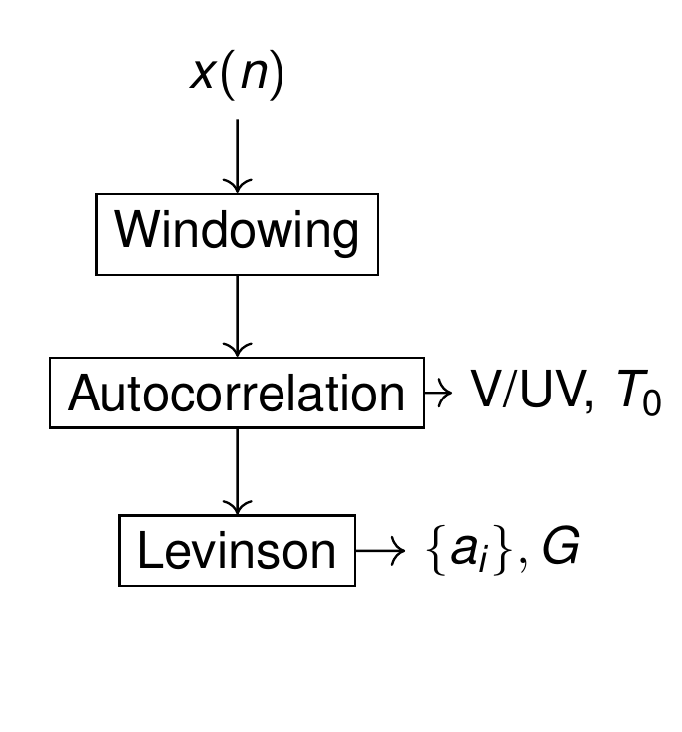
\includegraphics[width=0.75\textwidth]{images/Linear_predictive_coding_-_analysis.png}
\caption{Linear predictive coding - analysis.png}
\end{figure}

\begin{itemize}
  \item \textbf{Analysis}:

\end{itemize}
\begin{figure}[H]
\centering
\begin{tikzpicture}[
    block/.style={draw, rectangle, minimum width=2.2cm, minimum height=0.8cm, align=center, rounded corners=3pt, fill=teal!10, draw=teal!50!black, font=\small},
    arrow/.style={-latex, thick, draw=teal!50!black}
]
    \node [block] (speech) {Speech frame\\($\sim 20$ ms)};
    \node [block, right=0.8cm of speech] (window) {Windowing};
    \node [block, right=0.8cm of window] (autocorr) {Autocorrelation};
    \node [block, right=0.8cm of autocorr] (levinson) {Levinson-Durbin /\\Yule-Walker};
    
    \node [block, below=1.0cm of levinson] (out) {LPC coefficients, gain,\\pitch, voiced/unvoiced};
    
    \draw [arrow] (speech) -- (window);
    \draw [arrow] (window) -- (autocorr);
    \draw [arrow] (autocorr) -- (levinson);
    \draw [arrow] (levinson) -- (out);
\end{tikzpicture}
\caption{LPC10 Speech Analysis Chain}
\label{fig:lpc_analysis}
\end{figure}

\begin{itemize}
  \item \textbf{Prediction model}:

\end{itemize}
$$
\hat{x}(n)=-\sum_{i=1}^{P}a_i x(n-i)
$$

\begin{itemize}
  \item \textbf{Residual}:

\end{itemize}
$$
y(n)=x(n)-\hat{x}(n)=\sum_{i=0}^{P}a_i x(n-i),\quad a_0=1
$$

\begin{itemize}
  \item \textbf{Voiced frames} $\rightarrow$ pitch-period excitation.
  \item \textbf{Unvoiced frames} $\rightarrow$ noise-like excitation.
  \item \textbf{LPC-10} $\rightarrow$ low bitrate, less natural than CELP because excitation is rigid.

\end{itemize}
\begin{questionbox}{Domanda 45}
(A\&S Comp.) Draw the scheme and describe the operation of the functional blocks of an MP3 encoder.
\end{questionbox}


\begin{itemize}
  \item \textbf{MP3} $\rightarrow$ perceptual audio codec.

\end{itemize}
\begin{figure}[H]
\centering
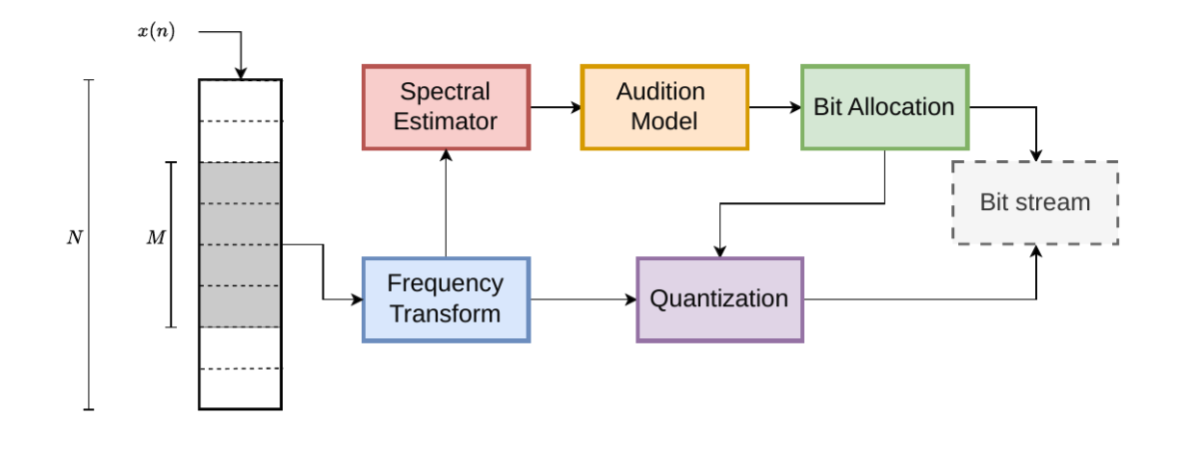
\includegraphics[width=0.75\textwidth]{images/Pasted_image_20260624185047.png}
\caption{Pasted image 20260624185047.png}
\end{figure}

\begin{itemize}
  \item \textbf{Main encoder chain}:

\end{itemize}
\begin{figure}[H]
\centering
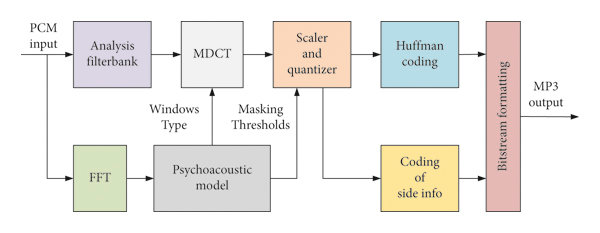
\includegraphics[width=0.75\textwidth]{images/Pasted_image_20260624213214.png}
\caption{Pasted image 20260624213214.png}
\end{figure}

\begin{itemize}
  \item \textbf{Functional blocks}:
  \begin{itemize}
    \item framing/windowing + transform/filterbank $\rightarrow$ convert time signal into spectral components;
    \item \textbf{psychoacoustic model} $\rightarrow$ estimate masking threshold from signal spectrum;
    \item \textbf{bit allocation} $\rightarrow$ spend more bits where ear is sensitive, fewer where noise is masked;
    \item \textbf{quantization} $\rightarrow$ lossy stage on spectral coefficients;
    \item \textbf{entropy coding} $\rightarrow$ final lossless compression stage.
  \end{itemize}
  \item \textbf{Psychoacoustic model} $\rightarrow$ encoder-side only; not needed at decoder.
  \item \textbf{Decoder} $\rightarrow$ entropy decoding, inverse quantization, inverse transform / synthesis filterbank.

\end{itemize}
\begin{questionbox}{Domanda 46}
(A\&S Comp.) Why are Line Spectrum Frequencies (LSF) preferred over direct quantization of LPC coefficients ($a_i$)?
\end{questionbox}


\begin{itemize}
  \item \textbf{Direct LPC coefficient quantization} $\rightarrow$ can create unstable synthesis filters.
  \item \textbf{LSF} $\rightarrow$ represent LPC filter through roots on unit circle.
  \item Stability condition easier to enforce by preserving interlacing/order:

\end{itemize}
$$
0<\omega_1^{(P)}<\omega_1^{(Q)}<\omega_2^{(P)}<\cdots<\pi
$$

\begin{itemize}
  \item \textbf{If quantization disturbs order} $\rightarrow$ decoder can restore valid ordering.

\end{itemize}
\begin{questionbox}{Domanda 47}
(A\&S Comp.) Regarding the Opus audio codec, what is the primary technical advantage of its hybrid design?
\end{questionbox}


\begin{itemize}
  \item \textbf{Opus} combines:
  \begin{itemize}
    \item \textbf{SILK} $\rightarrow$ LPC-based, efficient for speech and low bitrates;
    \item \textbf{CELT} $\rightarrow$ MDCT-based, efficient for music/general audio and low delay.
  \end{itemize}
  \item \textbf{Advantage} $\rightarrow$ seamless adaptation across speech/music, bitrate, latency; useful for WebRTC.

\end{itemize}
\begin{questionbox}{Domanda 48}
(A\&S Comp.) Which of the following best describes current research trends in the future of multimedia audio coding?
\end{questionbox}


\begin{itemize}
  \item Neural speech/audio codecs at very low bitrates.
  \item Perceptual and QoE-driven quality metrics.
  \item Spatial/immersive audio.
  \item Robust real-time coding under latency constraints.
  \item Quality assessment for generated/enhanced audio.

\end{itemize}
---

